\documentclass{article}
\newcounter{rownumbers}
\newcommand\rownumber{\stepcounter{rownumbers}\arabic{rownumbers}}
%\usepackage[a4paper, total={6in, 8in}]{geometry}
\usepackage{graphicx}
\usepackage{bm}
\usepackage{amsmath,amsfonts,mathtools}
\usepackage{amsthm}
\newtheorem{theorem}{Theorem}[section]
\newtheorem{lemma}[theorem]{Lemma}

\graphicspath{ {E:\College\Sem-6\PSP\CODES\TeX\Assignment-3} }
\usepackage{geometry}
 \geometry{
 a4paper,
 total={210mm,297mm},
 left=20mm,
 right=20mm,
 top=-2mm,
 bottom=2mm,
 }
 
%\usepackage[margin=0.5in]{geometry}

\usepackage{amsmath,amssymb}
\usepackage{ifpdf}
%\usepackage{cite}
\usepackage{algorithmic}
\usepackage{array}
\usepackage{mdwmath}
\usepackage{pdfpages}
\usepackage{mdwtab}
\usepackage{eqparbox}
\usepackage{parskip}
%\onecolumn
%\input{psfig}
\usepackage{color}
\usepackage{graphicx}
\setlength{\textheight}{23.5cm} \setlength{\topmargin}{-1.05cm}
\setlength{\textwidth}{6.5in} \setlength{\oddsidemargin}{-0.5cm}
\renewcommand{\baselinestretch}{1}
\pagenumbering{arabic}
\linespread{1.15}
\begin{document}
\textbf{
\begin{center}
{
\large{School of Engineering and Applied Science (SEAS), Ahmedabad University}\vspace{5mm}
}
\end{center}
%
\begin{center}
\large{Probability and Stochastic Processes (MAT277)\\ \vspace{4mm}
Homework Assignment-3\\\vspace{2mm}
Enrollment No: AU2140096 \hspace{4cm} Name: Ansh Virani }
\end{center}}
\vspace{2mm}


\vspace{10mm}

\begin{enumerate}
\item 
    Consider that Alice and Bob have no first girl child then they have \(k\) children as mentioned in the question. So, the probability for no girl child is \( \left(\cfrac{1}{2^k}\right)\).\\\\
    When they have one girl the probability is the complement of no girl child,\\
    \[
    \left(1 - \cfrac{1}{2^k}\right)
    \]
    The first \( i^{th} \) offspring are usually boys, that is to have at least \( i \geq 1 \) the probability is \( \cfrac{1}{2^i} \).\\
    Therefore, the predicted number of male children has increased as
    \[
    \sum_{i=1}^k \left(\cfrac{1}{2^i}\right) = \left(1 - \cfrac{1}{2^k}\right)
    \]
    \[
        \boxed{\therefore\ \textnormal{The expected number of female or male children is same that is } \left(1 - \cfrac{1}{2^k}\right).}
    \]
\newpage
\item 
\begin{enumerate}
    \item 
    \textbf{Maximizing the expected amount of money:}\\
    Given that the commodity sells for \$2 per ounce now, we have \$1000 to spend. \\
    Therefore, we can buy 
    \[ 
    \cfrac{1,000}{2} = 500 \text{ ounces}
    \]
    After one week, the price of the commodity can either increase to \$4 per ounce or decrease to \$1 per ounce. Both possibilities are equally likely.\\
    \begin{enumerate}
        \item If the price increases to \$4 per ounce:
        \begin{itemize}
            \item we have 500 ounces.
            \item Selling them at \$4 per ounce would give us \( 500 \times 4 = \$2,000. \)
        \end{itemize}
        \item If the price decreases to \$1 per ounce:
        \begin{itemize}
            \item we still have 500 ounces.
            \item Selling them at \$1 per ounce would give us \( 500 \times 1 = \$500. \)
        \end{itemize}
    \end{enumerate}
    Since both the scenarios are equally likely to occur, we calculate the expected value by taking the average of the possible outcomes:
    \[
        E [\text{Money at the end of the week}] = \cfrac{2,000 + 500}{2} = \$1,250
    \]
    \[
        \boxed{\therefore\ \textnormal{Our expected amount of the commodity at the end of the week will be \(\approx\) 1,250 ounces.}}
    \]
    \item \textbf{Maximizing the expected amount of the commodity at the end of the wek:}\\
    We should wait until the end of the week to buy because the price will either be \$1 or \$4 per ounce with equal probability.\\\\
    Therefore, calculating the expected price at the end of the week by taking average we get, \$2.50 per ounce.\\    
    With the given amount, we can buy
    \[
    \cfrac{1,000}{2.50} = 400 \text{ ounces}
    \]
    \[
        \boxed{\therefore\ \textnormal{Our expected amount of the commodity at the end of the week will be 400 ounces.}}
    \]
    Hence, if our objective is to maximize the expected amount of money, we should buy the commodity now and hold onto it.\\\\
    That strategy ensures us obtain the most commodity for your money, taking into account the uncertainty that can take place within the price fluctuations.\\
    \end{enumerate}

\newpage
\item 
    Let, the variable \( X \) denotes the player's winnings. The probability that the player wins their \( n^{th} \) game is given by \( \left(\cfrac{1}{2}\right)^n \).\\
    Calculating the Expectation:
        \begin{align*}
        E [X] &= \sum_{i=1}^{\infty} X P(X = X) \\\\
            &= \sum_{i=1}^{\infty} \left[2^n\cdot \left(\cfrac{1}{2}\right)^n\right] \\\\
            &= \sum_{i=1}^{\infty} (1) \\\\
            &= \infty
        \end{align*}
        \begin{enumerate}
            \item 
            No, I would not be pay \$1 million to play this game once.\\
            Considering the best case scenario: \$1 million to play once and you win in the first toss, you will take home a big amount \$2 million. But on the other hand, if you lose the bet, you will lose the invested amount.(\textit{Not a small amount})\\\\
            \textit{The fact \( E[X] = \infty \) is the expected value in the long run, not for one game.}\\
            \item 
            Yes, the expectation when considering a long run is indeed "something large," so we can expect the profit. Therefore, one can pay \$1 million for each game.
        \end{enumerate}

\newpage
\item 
    From the properties of expectation,    
    \[
        E[a] = a, \quad \text{here } a \text{ is a constant.}
    \]
    \[
        E[a - X] = a - E[X], \quad \text{here } X \text{ is a random variable.}
    \]
    Consider any constant function \( y \) as function of random variable \( X \) as below.
    \begin{align*}
        y = (X - E[X])^k \quad \ldots (1)
    \end{align*} 
    Expand R.H.S of eq.(1) using Binomial's expansion,
    \begin{align*}
        (X - E[X])^k 
        &= \binom{k}{0}X^k(-E[X])^0 + \binom{k}{1}X^{k-1}(-E[X])^1 + \ldots + \binom{k}{k}X^0(-E[X])^k \\
        &= X^k + (-E[X])^k - \binom{k}{1}X^{k-1}(E[X]) + \ldots + (-E[X])^k
    \end{align*}
    substituting these values in eq.(1),
    \begin{equation*}
        y - X^k = (E[X])^k - \binom{k}{1}X^{k-1}(E[X]) + \ldots + \binom{k}{k-1}X(-E[X])^{k-1} \hspace{20mm}\ldots (2)
    \end{equation*} 
    Apply expectation on both sides of eq.(2),
    \begin{equation*}
        E[y - X^k] = E\left[(E[X])^k - \binom{k}{1}X^{k-1}(E[X]) + \ldots + \binom{k}{k-1}X(-E[X])^{k-1}\right] \hspace{10mm}\ldots (3)
    \end{equation*}  
    On applying properties of expectation from the eq.(3), 
    \begin{equation*}
        E[X^k] = (E[X])^k - \binom{k}{1}E[X^{k-1}(E[X])] + \ldots + \binom{k}{k-1}E[X(-E[X])^{k-1}] \hspace{15mm}\ldots (4)
    \end{equation*}
    From the above eq.(4) it is interpreted that,
    \begin{equation*}
        (E[X^k]) > (E[X])^k
    \end{equation*}
    \textit{Hence, proved.}

\newpage
\item
    \begin{enumerate}
        \item
            It is given that the length of the streaks is
            \[ 
                k = \cfrac{\log_{2}{n+1}}{2} \text{ where } n \text{ is some power of 2.} 
            \]
            Consider the length of streaks be denoted by \(k\) and \(Y_i\) be that term of sequence of flips which 
            represents \(1\) whenever the streak of length \(k\) starts from the \(i\)-th flip.\\\\
            The length of the streak will be \( k \) from the \(i\)-th flip if the flips \(Y_i's\) are all same for \(i = 1,\ldots,n-k+1\).
            therefore
            \[ 
                \sum_{i=1}^{n-k+1} Y_i
            \]
            will be the total number of streaks of length \(k\).\\
            linearity of expectations states that
            \[
                E\left[\sum_{i=1}^{n-k+1} Y_i\right] = \sum_{i=1}^{n-k+1} E[Y_i] = \sum_{i=1}^{n-k+1} Pr(Y_i = 1).
            \]
            The \( Y_i \) will have value 1 if \( k-1 \) flips produce the same result as \( X_i \). Since the dealt coin is fair and flips are independent, the probability that \( Y_i \) is 1 will be
            \[
                Pr(Y_i = 1) = \left(\cfrac{1}{2}\right)^{k-1}.
            \]
            Hence, the value is,
            \[
                E\left[\sum_{i=1}^{n-k+1} Y_i\right] = \sum_{i=1}^{n-k+1} \left(\cfrac{1}{2}\right)^{k-1}.
            \]
            substituting, \( \log_{2}{n+1} \) for \( k \)
            \begin{align*}
                E\left[\sum_{i=1}^{n-k+1} Y_i\right] &= \sum_{i=1}^{n-k+1} \left(\cfrac{1}{2}\right)^{\log_2 n}\\
                &= \sum_{i=1}^{n-k+1} \left(\cfrac{1}{2^{\log_2 n}}\right)\\
                &= \sum_{i=1}^{n-k+1} \cfrac{1}{n}\\
                &= \cfrac{n-k+1}{n}\\
                &= \cfrac{n - \log_2 n - 1 + 1}{n}\\
                &= 1 - \cfrac{\log_2 n}{n}
            \end{align*}
            Since \(\cfrac{\log_2 n}{n}\) is of order 1, the expected number of streaks of order \(k\) is \(1 - o(1)\) with respect to \(n\).\\\\
            \textit{Hence, proved.}
        \newpage
        \item 
            Let \(n\) be the number of terms in the sequence of flips and the length of streaks be denoted by \(k\).\\\\
            If they are grouped into distinct blocks of \(k\) consecutive flips, then there will be \(\cfrac{n}{k}\) such blocks.\\\\
            Let \(E_1\) be the event that the sequence of \(n\) terms does not have any streaks of length \(k\) and \(E_2\) be the event that none of the blocks have a streak of length \(k\).\\\\
            It is easy to observe that \(E_1\) is possible if \(E_2\) holds, that is if none of the blocks have the streaks of length \(k\) then sequence will also not have any such streak.\\\\
            Therefore, \(Pr(E_1) \leq Pr(E_2)\).\\\\
            Since the coin is fair and flips are independent, the probability that a block of \(k\) consecutive flips has a streak of length \(k\) will be \(\left(\cfrac{1}{2}\right)^{k-1}\). Therefore, the probability that a block does not have any streak of length \(k\) is \(\left[1 - \left(\cfrac{1}{2^{k-1}}\right)\right]\).\\
            As there are \(\cfrac{n}{k}\) blocks,
            \[
                Pr(E_2) = \left(1 - \cfrac{1}{2^{k-1}}\right)^{\cfrac{n}{k}}.
            \]            
            Using the facts that \( k = 1 \leq \log_2 n - 2\log_2\log_2 n \), \( \cfrac{n}{k} \leq \cfrac{n}{\log_2 n} \), and \( 1 - x \leq e^{-x} \) and substituting them in the equation of the probability of \( E_2 \).            
            \begin{align*}
                Pr(E_2) &\leq \left(1 - \cfrac{1}{2^{(\log_2 n - 2\log_2\log_2 n)}}\right)^{\cfrac{n}{\log_2 n}}\\
                &= \left(\cfrac{\log_2^2 n}{n}\right)^{\cfrac{n}{\log_2 n}-1}\\
                &\leq \exp\left[-\cfrac{n}{\log_2 n}\left(\cfrac{\log_2^2 n}{n}\right)\right]\\
                &= \exp\left[-\log_2 n \left(\cfrac{\log_2 n}{n} \left(\log_2 n - 1\right)\right)\right]\\
                Pr(E_2) &= \exp\left[-\log_2 n \left(1 - \cfrac{\log_2 n}{n}\right)\right]
            \end{align*}            
            It is obtained that \(Pr(E_2) = \exp\left[-\log_2 n \left(1 - \cfrac{\log_2 n}{n}\right)\right]\).\\
            Simplifing further using the properties of logarithmic function, we get:
            \begin{align*}
                Pr(E_2) &= \exp\left[-\log_2 n \left(1 - \cfrac{\log_2 n}{n}\right)\right]\\
                &\leq \exp\left(-\log_2 n \left(\cfrac{1}{\log_2 e}\right)\right)\\
                &= \exp\left(\cfrac{\log_2 n}{\log_2 e}\right)\\
                &= \exp(-\ln n)
            \end{align*}
            It follows that
            \[
                Pr(E_2) \leq \cfrac{1}{n}.
            \]
            \textit{Hence, it is proved that}
            \[
                \mathbf{Pr(\textbf{no streak of length at least }[\log_2 n - 2\log_2 \log_2 n]) < \cfrac{1}{n}}.
            \]
    \end{enumerate}

\newpage
\item 
    \begin{enumerate}
    \item 
        Let \(f\) be a convex function on the interval I. If \(x_1, x_2, \ldots, x_n \in I\) and \(\lambda_1, \lambda_2, \ldots, \lambda_n\) are non negative real numbers such that \(\sum_{i=1}^{n} \lambda_i = 1\), then
        \[
            f\left(\sum_{i=1}^{n} \lambda_i x_i\right) \leq \sum_{i=1}^{n} \lambda_i f(x_i).
        \]
        The case for \(n = 2\) is true by the definition of convex. Assume the relation holds for \(n\), then we have
        \begin{align*}
            f\left(\sum_{i=1}^{n+1} \lambda_i x_i\right) &= f\left(\sum_{i=1}^{n} \lambda_i x_i + \lambda_{n+1}x_{n+1}\right)
            = f\left(\lambda_{n+1}\cdot x_{n+1} + (1 - \lambda_{n+1}) \cfrac{1}{1 - \lambda_{n+1}}\sum_{i=1}^{n} \lambda_i x_i\right)\\
            &\leq \lambda_{n+1}\cdot f(x_{n+1}) + (1 - \lambda_{n+1})\cdot f\left(\cfrac{1}{1 - \lambda_{n+1}}\sum_{i=1}^{n} \lambda_i x_i\right)\\
            &= \lambda_{n+1}\cdot f(x_{n+1}) + (1 - \lambda_{n+1})\cdot f\left(\sum_{i=1}^{n} \cfrac{\lambda_i}{1 - \lambda_{n+1}}\cdot x_i\right)\\
            &\leq \lambda_{n+1}\cdot f(x_{n+1}) + (1 - \lambda_{n+1})\cdot \sum_{i=1}^{n} \cfrac{\lambda_i}{1 - \lambda_{n+1}}\cdot f(x_i)\\
            &= \sum_{i=1}^{n} \lambda_i\cdot f(x_i) + \lambda_{n+1}\cdot f(x_{n+1})\\
            &= \sum_{i=1}^{n+1} \lambda_i f(x_i).
        \end{align*} 
        \textit{Hence, by induction, the theorem is proven.}\\
    \item 
        We all know that expectation is denoted by:
        \begin{align*}
            E[X] &= \sum_{i=1}^{n} X_i P(X_i) \\
        \end{align*}
        Since, \(P(X_i)\geq 0\), let \(\lambda_i = P(X_i)\geq 0\) \& \(\sum_{i=1}^{n} P(X_i) = 1\)\\\\
        \begin{align*}
            \therefore 
            f(E[X]) &= f\left(\sum_{i}^{n}x_i P(X_i)\right)\\
            &= f\left(\sum_{i}^{n}X_i \lambda_i\right) \leq \sum_{i}^{n}\lambda_i f(X_i)\\
            &= \sum_{i}^{n}p(X_i) f(X_i)\leq E[f(X)]
        \end{align*}
        \textit{Hence, Proved}
    \end{enumerate}

\newpage
\item
    \begin{enumerate}
    \item 
        \begin{enumerate}
        \item
            To find \(\mathbf{E[(4X - 1)^2]}\), we can use the properties of expected value.
            \begin{align*}
                E[(4X - 1)^2] = E[16X^2 - 8X + 1]
            \end{align*}
            \textit{By using linearity of expectation:}
            \begin{align*}
                E[16X^2 - 8X + 1] = 16E[X^2] - 8E[X] + E[1]
            \end{align*}
            We know that,
            \begin{align*}
                Var(X) = E[X^2] - (E[X])^2\\
                \therefore E[X^2] = Var(X) + (E[X])^2
            \end{align*}
            substituting this into the expression,we get:
            \begin{align*}
                16(Var(X) + (E[X])^2) - 8E[X] + 1 &= 16(1 + 3^2) - (8 \times 3) + 1 = 16(10) - 24 + 1\\
                &= 160 - 24 + 1 = 137
            \end{align*}
            \[
                \boxed{\therefore E\left[(4X - 1)^2\right] = 137}
            \]
        \item
            Now, let's find \(\mathbf{Var(5 - 2X)}\):
            \begin{align*}
                E[5 - 2X] = 5 - 2E[X]\\
                5 - (2 \times 3) = 5 - 6 = -1
            \end{align*}
            \begin{align*}
                Var(5 - 2X) &= E[(5 - 2X)^2] - [E(5 - 2X)]^2\\
                &= E[25 - 20X + 4X^2] - (-1)^2
            \end{align*}
            Using the properties of expectation:
            \begin{align*}
                25 - 20E[X] + 4E[X^2] - 1 &= 25 - (20 \times 3) + (4 \times 10) - 1
                \\ &= 25 - 60 + 40 - 1 = 4
            \end{align*}
            \[
                \boxed{\therefore Var(5 - 2X) = 4}
            \]\\
        \end{enumerate}
    \item
        The total number of selecting 2 cards from a deck of 52 cards is given by: \(n(T)\) = \(\binom{52}{2}\) = 1326.\\\\
        Now, considering both the selected cards are of the same suit: \(n(ss)\) = \(\binom{4}{1}\).\(\binom{13}{2}\) = 312.\\\\
        Similarly, if both the selected cards are of the same color: \(n(sc)\) = \(\binom{2}{1}\).\(\binom{26}{2}\) = 650.\\\\
        \begin{align*}
            \therefore Pr(ss) = \cfrac{312}{1326} \approx 0.2353\\
            \therefore Pr(sc) = \cfrac{650}{1326} \approx 0.4902\\
        \end{align*}
        \(\therefore \textnormal{It implies that} P(X=1) = Pr(sc)\)\ ...[the player won \$1]\\
        \(\therefore \textnormal{It implies that} P(X=2) = Pr(ss)\)\ ...[the player won \$2]\\\\
        For other cases, it's given that a player will lose \$0.50
        \begin{align*}
        \therefore P(X= -0.50) &= 1 - P(X=1) - P(X=2)\\
        &= 1- [0.2353 + 0.4902]\\
        &= 0.2745
        \end{align*}
        We know that,
        \begin{align*}
            Var(X) = E[X^2] - (E[X])^2\ \ \ \ \ \ ...(i)\\
            E[X^2] = \sum x^2.P(X=x)\ \ \& \ \ E[X] = \sum x.P(X=x)
        \end{align*}
        \begin{align*}
            \therefore  E[X^2] &= (2^2\times 0.2353) + (1^2\times 0.4902) + (-0.5^2\times 0.2745)\\
            &= 1.5
        \end{align*}
        \begin{align*}
            \therefore  E[X] &= (2\times 0.2353) + (1\times 0.4902) + (-0.5\times 0.2745)\\
            &= 0.8235
        \end{align*}
        \begin{align*}
            Var(X) &= E[X^2] - (E[X])^2\\
            &= 1.5 - (0.8235^2)\\
            &= 0.8218
        \end{align*}
        \(\therefore\) The variance of the amount won by the player is, \$0.8218.\\
    \item
        Let's say we have two teams A \& B.\\
        If Team A has a winning Probability of \(p\), then winning probability of Team B will be \((1-p)\).
        Let \(N\) be total number of games played when \(i=2\).\\
        Hence, \(N\) can take only two values \(i.e,\) 2 OR 3 (Since for atleast one of them to win, atmost 3 games are required).\\
        \(P(N=2) = P(N=2, A\ wins) + P(N=2, B\ wins)\)\\
        \(= p^2 + (1-p)^2\)\\\\
        \(P(N=3) = P(N=3, A\ wins) + P(N=3, B\ wins)\)\\
        $\bullet$ For A to win when \(N=3\), A has to win the \(3^{rd}\) game and any of the first two games.\\\\
        \(\therefore P(N=3, A\ wins) = p.(1-p).p + (1-p).p.p\)\\
        \(=2.p^2.(1-p)\)\\\\
        $\bullet$ Similarly for B to win when\(N=3\), we get:\\\\
        \(\therefore P(N=3, B\ wins) = p.(1-p).(1-p) + (1-p).p.(1-p)\)\\
        \(=2.p.(1-p)^2\)\\\\
        We get the Expectation:
        \begin{align*}
            E[N] &= 2.P(N=2) + 3.P(N=3)\\
            &= \left[2.\left(p^2 + (1-p)^2\right)\right] + \left[3.\left(2p^2(1-p) + 2p(1-p)^2\right)\right]\\
            &= -2p^2 + 2p + 2
        \end{align*}
        Similarly,
        \begin{align*}
            E[N^2] &= 2^2.P(N=2) + 3^2.P(N=3)\\
            &= \left[4.\left(p^2 + (1-p)^2\right)\right] + \left[9.\left(2p^2(1-p) + 2p(1-p)^2\right)\right]\\
            &= -10p^2 + 10p + 4
        \end{align*}
        The variance can we calculated by,
        \begin{align*}
            Var(N) &= E[N^2] - (E[N])^2\\
            &= \left[-10p^2 + 10p + 4\right] - \left[-2p^2 + 2p + 2\right]^2\\
            &= -4p^4 + 8p^3 - 6p^2 + 2p
        \end{align*}

        $\bullet$ \textbf{The \(2^{nd}\) part can't be proved as the value of probability can't be more than 1 (we are given 12).}
    \end{enumerate}

\newpage
\item
    \begin{enumerate}
        \item 
        Determine the value of 
        \[ 
            Pr\left(\cfrac{1}{2} \leq X \leq \cfrac{3}{4}\right) \text{ and } Pr\left(X \leq \cfrac{1}{2}\  \middle| \ \cfrac{1}{4} \leq X \leq \cfrac{3}{4}\right)
        \]\\
        We know that \(X\) be a uniform random variable on [0,1]. Thus,
        The density function of \(X\) is given as follows:
        \[ 
            f(x) = 1, \quad 0 < x < 1 
        \]
        Conditional probability for continuous random variable is defined as
        \[ 
            Pr(E|F) = \cfrac{Pr(E \cap F)}{Pr(F)} 
        \]
        Substitute \( E = X \leq \cfrac{1}{2} \) and \( F = \cfrac{1}{4} \leq X \leq \cfrac{3}{4} \) in 
        \[ 
            Pr(E|F) = \cfrac{Pr(E \cap F)}{Pr(F)}
        \]
        as follows:
        \begin{align*}
            Pr\left(X \leq \cfrac{1}{2}\  \middle| \ \cfrac{1}{4} \leq X \leq \cfrac{3}{4}\right) &= \cfrac{Pr\left(\left(X \leq \cfrac{1}{2}\right)\cap \left(\cfrac{1}{4} \leq X \leq \cfrac{3}{4}\right)\right)}{Pr\left(\cfrac{1}{4} \leq X \leq \cfrac{3}{4}\right)}\\\\
            &= \cfrac{Pr\left(\cfrac{1}{4} \leq X \leq \cfrac{1}{2}\right)}{Pr\left(\cfrac{1}{4} \leq X \leq \cfrac{3}{4}\right)}
        \end{align*}
        It is known that the probability of the interval \( [a,b] \) is given by the integral
        \[ 
            Pr(a \leq X \leq b) = \int_a^b f(x) \ dx 
        \]
        applying this to find the probability of the interval [a,b]:
        \begin{align*}
            Pr\left(X \leq \cfrac{1}{2}\ \middle| \ \cfrac{1}{4} \leq X \leq \cfrac{3}{4}\right) &= \cfrac{\int_{1/4}^{1/2} 1 \ dx}{\int_{1/4}^{3/4} 1 \ dx}\\
            &= \cfrac{\left[ x \right]_{1/4}^{1/2}}{\left[ x \right]_{1/4}^{3/4}}\\
            &= \cfrac{1}{2}
        \end{align*}
        substituting \( E = X \leq \cfrac{1}{4} \) and \( F = \cfrac{1}{3} \leq X \leq \cfrac{2}{3} \) in
        \[ 
            Pr(E|F) = \cfrac{Pr(E \cap F)}{Pr(F)}
        \]
        \begin{align*}
            Pr\left( X \leq \cfrac{1}{4}\ \middle| \ X \leq \cfrac{1}{3} \right) &= \cfrac{Pr\left(\left(X \leq \cfrac{1}{4}\right) \cap \left(\left(X \leq \cfrac{1}{3}\right) \cup \left(X \geq \cfrac{2}{3}\right) \right) \right)}{Pr\left( \left(X \leq \cfrac{1}{3}\right) \cup \left(X \geq \cfrac{2}{3}\right) \right)}\\ 
            &= \cfrac{Pr\left( X \leq \cfrac{1}{4} \right)}{Pr\left( \left(X \leq \cfrac{1}{3}\right) \cup \left(X \geq \cfrac{2}{3}\right) \right)}
        \end{align*}
        We know that \( Pr(A \cup B) = Pr(A) + Pr(B) - Pr(A \cap B) \).

        Here 
        \[ 
            Pr\left( \left( X \leq \cfrac{1}{3} \right) \cap \left( X \geq \cfrac{2}{3} \right) \right) = 0
        \]
        so,
        \[ 
            {Pr\left( \left(X \leq \cfrac{1}{3}\right) \cup \left(X \geq \cfrac{2}{3}\right) \right)} = Pr\left( X \leq \cfrac{1}{3} \right) + Pr\left( X \geq \cfrac{2}{3} \right)
        \]
        \[ 
            Pr\left( X \leq \cfrac{1}{4}\  \middle| \ \left( X \leq \cfrac{1}{3} \right) \cup \left( X \geq \cfrac{2}{3} \right) \right) = 
            \cfrac{Pr\left( X \leq \cfrac{1}{4} \right)}{Pr\left( X \leq \cfrac{1}{3} \right) + Pr\left( X \geq \cfrac{2}{3} \right)} 
        \]\\
        It is known that the probability of the interval \( [a,b] \) is given by the integral 
        \[ 
            Pr(a \leq X \leq b) = \int_{a}^{b} f(x) \ dx 
        \]
        \begin{align*} 
            Pr\left( X \leq \cfrac{1}{4} \middle| \left( X \leq \cfrac{1}{3} \right) \cup \left( X \geq \cfrac{2}{3} \right) \right) &= 
            \cfrac{\int_{0}^{1/4} 1 \ dx}{\int_{0}^{1/3} 1 \ dx + \int_{2/3}^{1} 1 \ dx} \\
            &= \cfrac{\left[ x \right]_{0}^{1/4}}{\left[ x \right]_{0}^{1/3} + \left[ x \right]_{2/3}^{1}}\\ 
            &= \cfrac{\cfrac{1}{4} - 0}{\left( \cfrac{1}{3} - 0 \right) + \left( 1 - \cfrac{2}{3} \right)} \\
            &= \cfrac{\cfrac{1}{4}}{\cfrac{1}{3} + \cfrac{1}{3}} \\\\
            &= \cfrac{\left(\cfrac{1}{4}\right)}{\left(\cfrac{2}{3}\right)} \\
            &= \cfrac{3}{8}\\ 
        \end{align*}
        Hence, the values are 

        \[ 
            \boxed{Pr\left( X \leq \cfrac{1}{4} \middle| X \leq \cfrac{1}{3} \right) = \cfrac{1}{2} \quad \text{and} \quad 
            Pr\left( X \leq \cfrac{1}{4} \middle| \left( X \leq \cfrac{1}{3} \right) \cup \left( X \geq \cfrac{2}{3} \right) \right) = \cfrac{3}{8}.}
        \]\\
    \item 
        Find the expected value of the \(k^{th}\) largest of the \(n\) random variables.\\
        The objective is to find \(E[\max\{x_1,x_2,\ldots,x_n\}]\)\\
        Therefore, 
        \begin{align*}
            F_{\max\{x_1,x_2,\ldots,x_n\}}(a) &= P(x_1 \leq a, x_2 \leq a, \ldots, x_n \leq a)\\
            &= F_x(a) F_x(a) \ldots F_x(a)\\
            &= (1-e^{\lambda_1 a})(1-e^{\lambda_2 a})...(1-e^{\lambda_n a})
        \end{align*}
        Now, since
        \begin{align*}
            E\left[F_{\max\{x_1,x_2,\ldots,x_n\}}\right] &= \int_0^\infty 1 - F_{\max\{x_1,x_2,\ldots,x_n\}}(a) \ da\\
            &= \int_0^\infty (1-e^{\lambda_1 a})(1-e^{\lambda_2 a})...(1-e^{\lambda_n a}) \ da\\
            &= \int_0^\infty 1 - (1-e^{a})(1-e^{a})...(1-e^{a}) \ da
        \end{align*}
        Since, parameter \(\lambda\) is 1, that is,
        \[
            \lambda_1 = \lambda_2 = \ldots = \lambda_n = 1
        \]
        This implies;
        \[
            \int_0^\infty (1 - (1-e^{a})^n) \ da = \int_0^\infty 1 - \left(1 - ne^{a} + \cfrac{n(n-1)e^{2a}}{2!} - \ldots - \cfrac{n(n-1)(n-r+1)(-e^{a})^r}{r!} + \ldots \infty\right)
        \]
        expanding the binomial expression,
        \[
            (1-x)^n = 1 + (-nx) + \cfrac{n(n-1)}{2}x^2 + \ldots + \cfrac{(-1)^r(n(n-1)\ldots(n-r+1))}{r!}x^r + \ldots \infty
        \]
        Therefore,
        \begin{align*}
            E[\max\{x_1,x_2,\ldots,x_n\}] &= \int_0^\infty ne^{a} - \cfrac{n(n-1)e^{2a}}{2!} + \ldots + \cfrac{(-1)^r(n(n-1))}{r!} - (n-r+1)e^{ar}\ da\\
            &= \left[ne^{a} - \cfrac{n(n-1)e^{2a}}{4} + \ldots + (-1)^r\cfrac{n(n-1) - (n-r+1)e^{ar}}{(rr!)}\right]_0^\infty\\
            &= \infty
        \end{align*}
    \item 
        It is known that one person must wait exactly for 15 minutes for the other person. So, the inequality when two people meet can be written as: \(|X - Y| \leq 15\).\\\\
        Consider that \(X\) and \(Y\) are random variables, which are independent and uniformly distributed on the interval \([0,60]\).\\\\
        The inequality is divided as follows:\\
        For the first 15 minutes, the probability is \(\left(y + \cfrac{1}{4}\right)\). For the next half an hour, the probability is \(\left(\cfrac{1}{2}\right)\) and for the next 15 minutes, the probability is \(\left(\cfrac{5}{4} - y\right)\).\\\\
        Therefore we calculate the required probability \(P(|X - Y| \leq 15)\):
        \begin{align*}
            P(|X - Y| \leq 15) &= \int_{-\infty}^{\infty} \int_{y-15}^{y+15} f_{X,Y}(x,y) \,dx\,dy\\
            &= \int_0^{y+15} \int_{y-15}^{y+15} f_{X}(x) f_{Y}(y) \,dx\,dy\\
            &= \int_0^{60}\int_{y-15}^{y+15} f_{X}(x) \,dx\,dy
        \end{align*}
        It is obtained from the problem that
        \[
            \int_{y-15}^{y+15} f_{X}(x) \,dx = 
            \begin{cases} 
            y + \cfrac{1}{4}, & 0 \leq y < 15 \\
            \cfrac{1}{2}, & 15 \leq y < 45 \\
            \cfrac{5}{4} - y, & 45 \leq y \leq 60 
            \end{cases}
        \]
        \begin{align*}
            P(|X - Y| \leq 15) &= \int_{0}^{15} \left(y + \cfrac{1}{4}\right) \,dy + \int_{15}^{45} \left(\cfrac{1}{2}\right) \,dy + \int_{45}^{60} \left(\cfrac{5}{4} - y\right) \,dy\\
            &= \cfrac{1}{2} \left(\cfrac{1}{4}\right)^2 + \left(\cfrac{1}{4}\right)^2 + \left(\cfrac{1}{4}\right) + \cfrac{1}{2} \left(\cfrac{1}{4}\right)^2 + \left(\cfrac{1}{4}\right)^2\\
            &= \cfrac{7}{16}
        \end{align*}
    \end{enumerate}

\newpage
\item
    \begin{figure}
        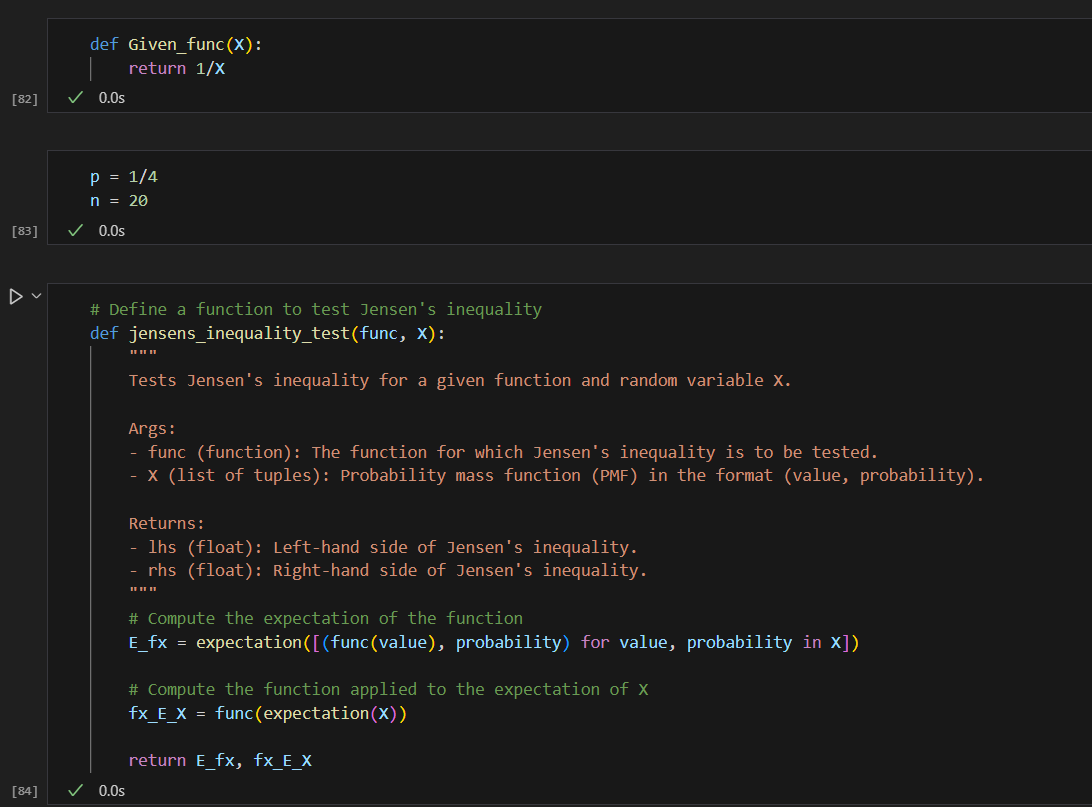
\includegraphics{1-1.png}
        \caption{Function}
    \end{figure}
    \begin{figure}
        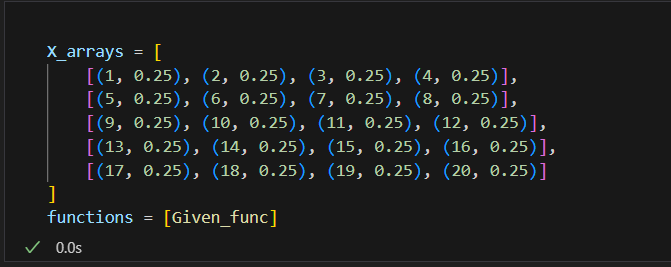
\includegraphics{1.png}
        \caption{PMF}
    \end{figure}
    \begin{figure}
        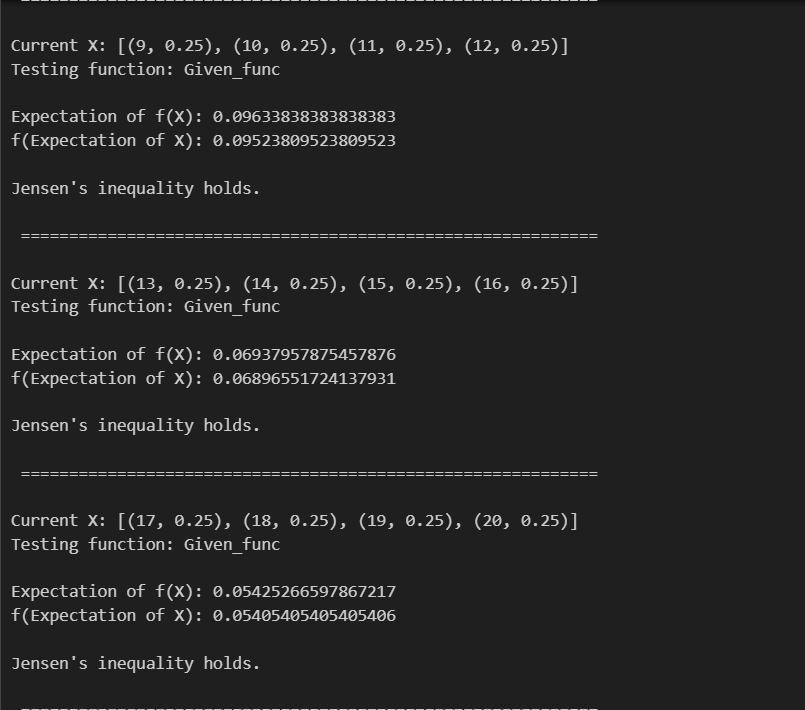
\includegraphics{3.png}
        \caption{Output}
    \end{figure}
\end{enumerate}
\end{document}